\documentclass[crop, tikz]{standalone}
\usepackage{tikz}
\usepackage{amssymb}
\usetikzlibrary{calc}
\usepackage{colortbl}

 
% Definition of circles
\def\firstcircle{(0,0) circle (1.5cm)}
\def\secondcircle{(0:2cm) circle (1.5cm)}
\def\innercircle{(-0.3,0) circle (0.8cm)}

\colorlet{circle edge}{black!80}
\colorlet{circle area}{gray!50}

\tikzset{filled/.style={fill=circle area, draw=circle edge, thick},
    outline/.style={draw=circle edge, very thick}}

\setlength{\parskip}{5mm}
 
 \begin{document}

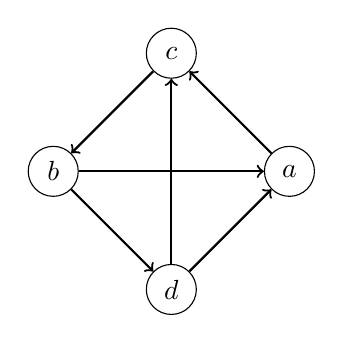
\begin{tikzpicture}

\node[circle,draw, minimum width=0.25in] at (0,0) (b) {$b$}; 
\node[circle,draw,minimum width=0.25in] at (3,0) (a) {$a$}; 
\node[circle,draw,minimum width=0.25in] at (1.5,1.5) (c) {$c$}; 
\node[circle,draw,minimum width=0.25in] at (1.5,-1.5) (d) {$d$}; 

\path[->,draw,thick] (b) to (a);
\path[->,draw,thick] (d) to (c);
\path[->,draw,thick] (c) to  (b);
\path[->,draw,thick] (a) to  (c);
\path[->,draw,thick] (d) to  (a);
\path[->,draw,thick] (b) to  (d);

\end{tikzpicture}
\end{document}



